%!TEX program = xelatex
\documentclass[11pt]{article}

\usepackage{polyglossia}
\setdefaultlanguage[variant=british]{english}
\setotherlanguage{dutch}

\usepackage{booktabs} % Required for prettier tables
\usepackage{multirow}

\usepackage{graphicx}
\usepackage{subfig}

\widowpenalties 1 10000 % Don't spread a paragraph across two pages but start it on the second page instead (no bastards) 
\raggedbottom

\usepackage{enumitem} % Required for list customisation
\setlist{noitemsep} % No spacing between list items

\usepackage{setspace}

\usepackage{geometry} % Required for adjusting page dimensions and margins
\geometry{
	paper=a4paper, % Paper size, change to letterpaper for US letter size
	top=2.5cm, % Top margin
	bottom=3cm, % Bottom margin
	left=3cm, % Left margin
	right=3cm, % Right margin
	headheight=0.75cm, % Header height
	footskip=1.5cm, % Space from the bottom margin to the baseline of the footer
	headsep=0.75cm, % Space from the top margin to the baseline of the header
	%showframe, % Uncomment to show how the type block is set on the page
}

\usepackage{xurl} % Tells latex how to line-break a url 
\usepackage{hyperref} % Allows for clickable and configurable urls

\hypersetup{
    colorlinks=true,
    linkcolor=black,
    citecolor=black,
    menucolor=black,
    urlcolor=cyan
    }
\urlstyle{same}



\begin{document}

\begin{titlepage}

\author{
    \LARGE G, Adamowicz, G, Todorević, \\
	\LARGE S, Karaduman, R, Roos \\ 
    \textsc{\small client: Michiel Ybema - MrFix} \\
}

\title{
	\vspace{80pt}
	\rule{\linewidth}{0.7pt}\\
	\vspace{7pt}
	\huge{Plan of Approach}\\
	\rule{\linewidth}{0.8pt}\\
	\vspace{30pt}
}

\date{\small \today}

\maketitle

\vspace{\fill}
\normalfont\small
\centering
\textsc{Bit Academy - ICT, Software Developer}\\
\vspace{10pt}

\thispagestyle{empty} % Don't print page number on this page
\end{titlepage}

\tableofcontents
\newpage

\section{Introduction}

This document is part of the project executed by students at the Bit Academy in Amsterdam, 
at the request of Michiel Ybema, representative of mrFix. MrFix is a company aiming to 
easily connect customers in need of home repair or improvement with trustworthy
professionals. The project's duration is one week. This project's mission is to:

\begin{enumerate}
	\item Analyse the various useflows within mrFix's services, and their competitors and 
		come up with a preliminary design for a mobile app.
	\item Build a minimal working prototype for a mobile app suitable for the business of 
		mrFix based on this design.
\end{enumerate}

Throughout this document the company of mrFix may be revered to as \textit{client}, users 
of the service as \textit{customers} and the people performing the jobs as 
\textit{fixers}.

\section{Prototype requirements}

The following requirements need to be taken into consideration when designing the 
prototype: 

\begin{itemize}
	\item Fixers need a publicly visible profile.
	\item The app needs to include an intuitive messaging system for communication between 
		customer and fixer.
	\item Customers need a clear and accurate quote, or at least estimation, for the cost 
		of the job.
	\item The app needs to facilitate making appointments between customers and fixers.
	\item Customers need certainty that the job will be done right the first time.
	\item Customers need certainty that the invoice matches the actual work done.
	\item The app needs to handle payments from the customer to the fixer.
	\item Customers need to be able to write reviews about their fixer.
\end{itemize}

\section{Project goals}

The client has voiced an interest in the following points: 

\begin{itemize}
	\item An overview of rival apps.
	\item Clear documentation provided along with the prototype.
	\item An overview of industry standard technologies useful for building the desired 
		product.
	\item An overview of third party Software-as-a-service providers and/or open source 
		libraries to use.
\end{itemize}

\section{Target audience}

The target audience for mrFix's service is primarily well-off people with limited time 
and/or DIY skills.

\section{User stories}

Each of these \textit{user stories} represent a feature or scenario that the customers 
would reasonably expect to be provided for in the app. 

\begin{table}[h]
	\begin{tabular}{llll} 
		\textbf{As a (role):} & \textbf{In order to:} & \textbf{I want:} \\
		\toprule
		client & 
			\begin{tabular}{@{}c@{}}offer the right experience \\
			to customers and fixers \end{tabular}  &
			\begin{tabular}{@{}c@{}}to have features tailored separately \\
			for fixers and customers \end{tabular} \\ 
		\midrule
		client & 
			\begin{tabular}{@{}c@{}}offer the right experience \\
			to customers and fixers \end{tabular}  &
			\begin{tabular}{@{}c@{}}to match fixers to customers \\
			effectively \end{tabular} \\ 
		\midrule
		customer & find a suitable fixer  &
			\begin{tabular}{@{}c@{}}to be able to create a post \\
			detailing the job I need fixed \end{tabular} \\
		\midrule
		Either fixer or customer & prevent missing appointments &
			\begin{tabular}{@{}c@{}}to be able to make appointments \\
				in an online calendar \end{tabular} \\ 
		\midrule
		Either fixer or customer & have clarity around payments &
			\begin{tabular}{@{}c@{}}to be able to submit and view \\
				quotes and cost estimations \end{tabular} \\ 
		\midrule
		Either fixer or customer & communicate clearly &
			\begin{tabular}{@{}c@{}}to have a messaging system to \\
			talk directly to my fixer/customer \end{tabular} \\ 
		\midrule
		customer & 
			\begin{tabular}{@{}c@{}}have insight in my \\
			previous job postings \end{tabular}  &
			\begin{tabular}{@{}c@{}}to have an overview of \\
			previously completed jobs \end{tabular} \\ 
		\midrule
		fixer & have insight in my job history &
			\begin{tabular}{@{}c@{}}to have an overview of \\
			previously completed jobs \end{tabular} \\ 
	\end{tabular}
\end{table}

\section{Planning}

The project kicked of on Monday, November 21 and will conclude on Friday 25th. 

\begin{table}[h]
	\centering
	\begin{tabular}{llll} 
		\toprule
		\textbf{Day 1} & exploratory research, \\
					   & write plan of approach, \\
		\textbf{Day 2} & UML useflow charts, \\
					   & job posting design  \\
		\textbf{Day 3} & fixer profile design \\
		\textbf{Day 4} & messaging design \\
		\textbf{Day 5} & demo \\
	\end{tabular}
\end{table}

\section{wireframe}

\begin{figure}[h]%
    \centering
    \subfloat[\centering home]{{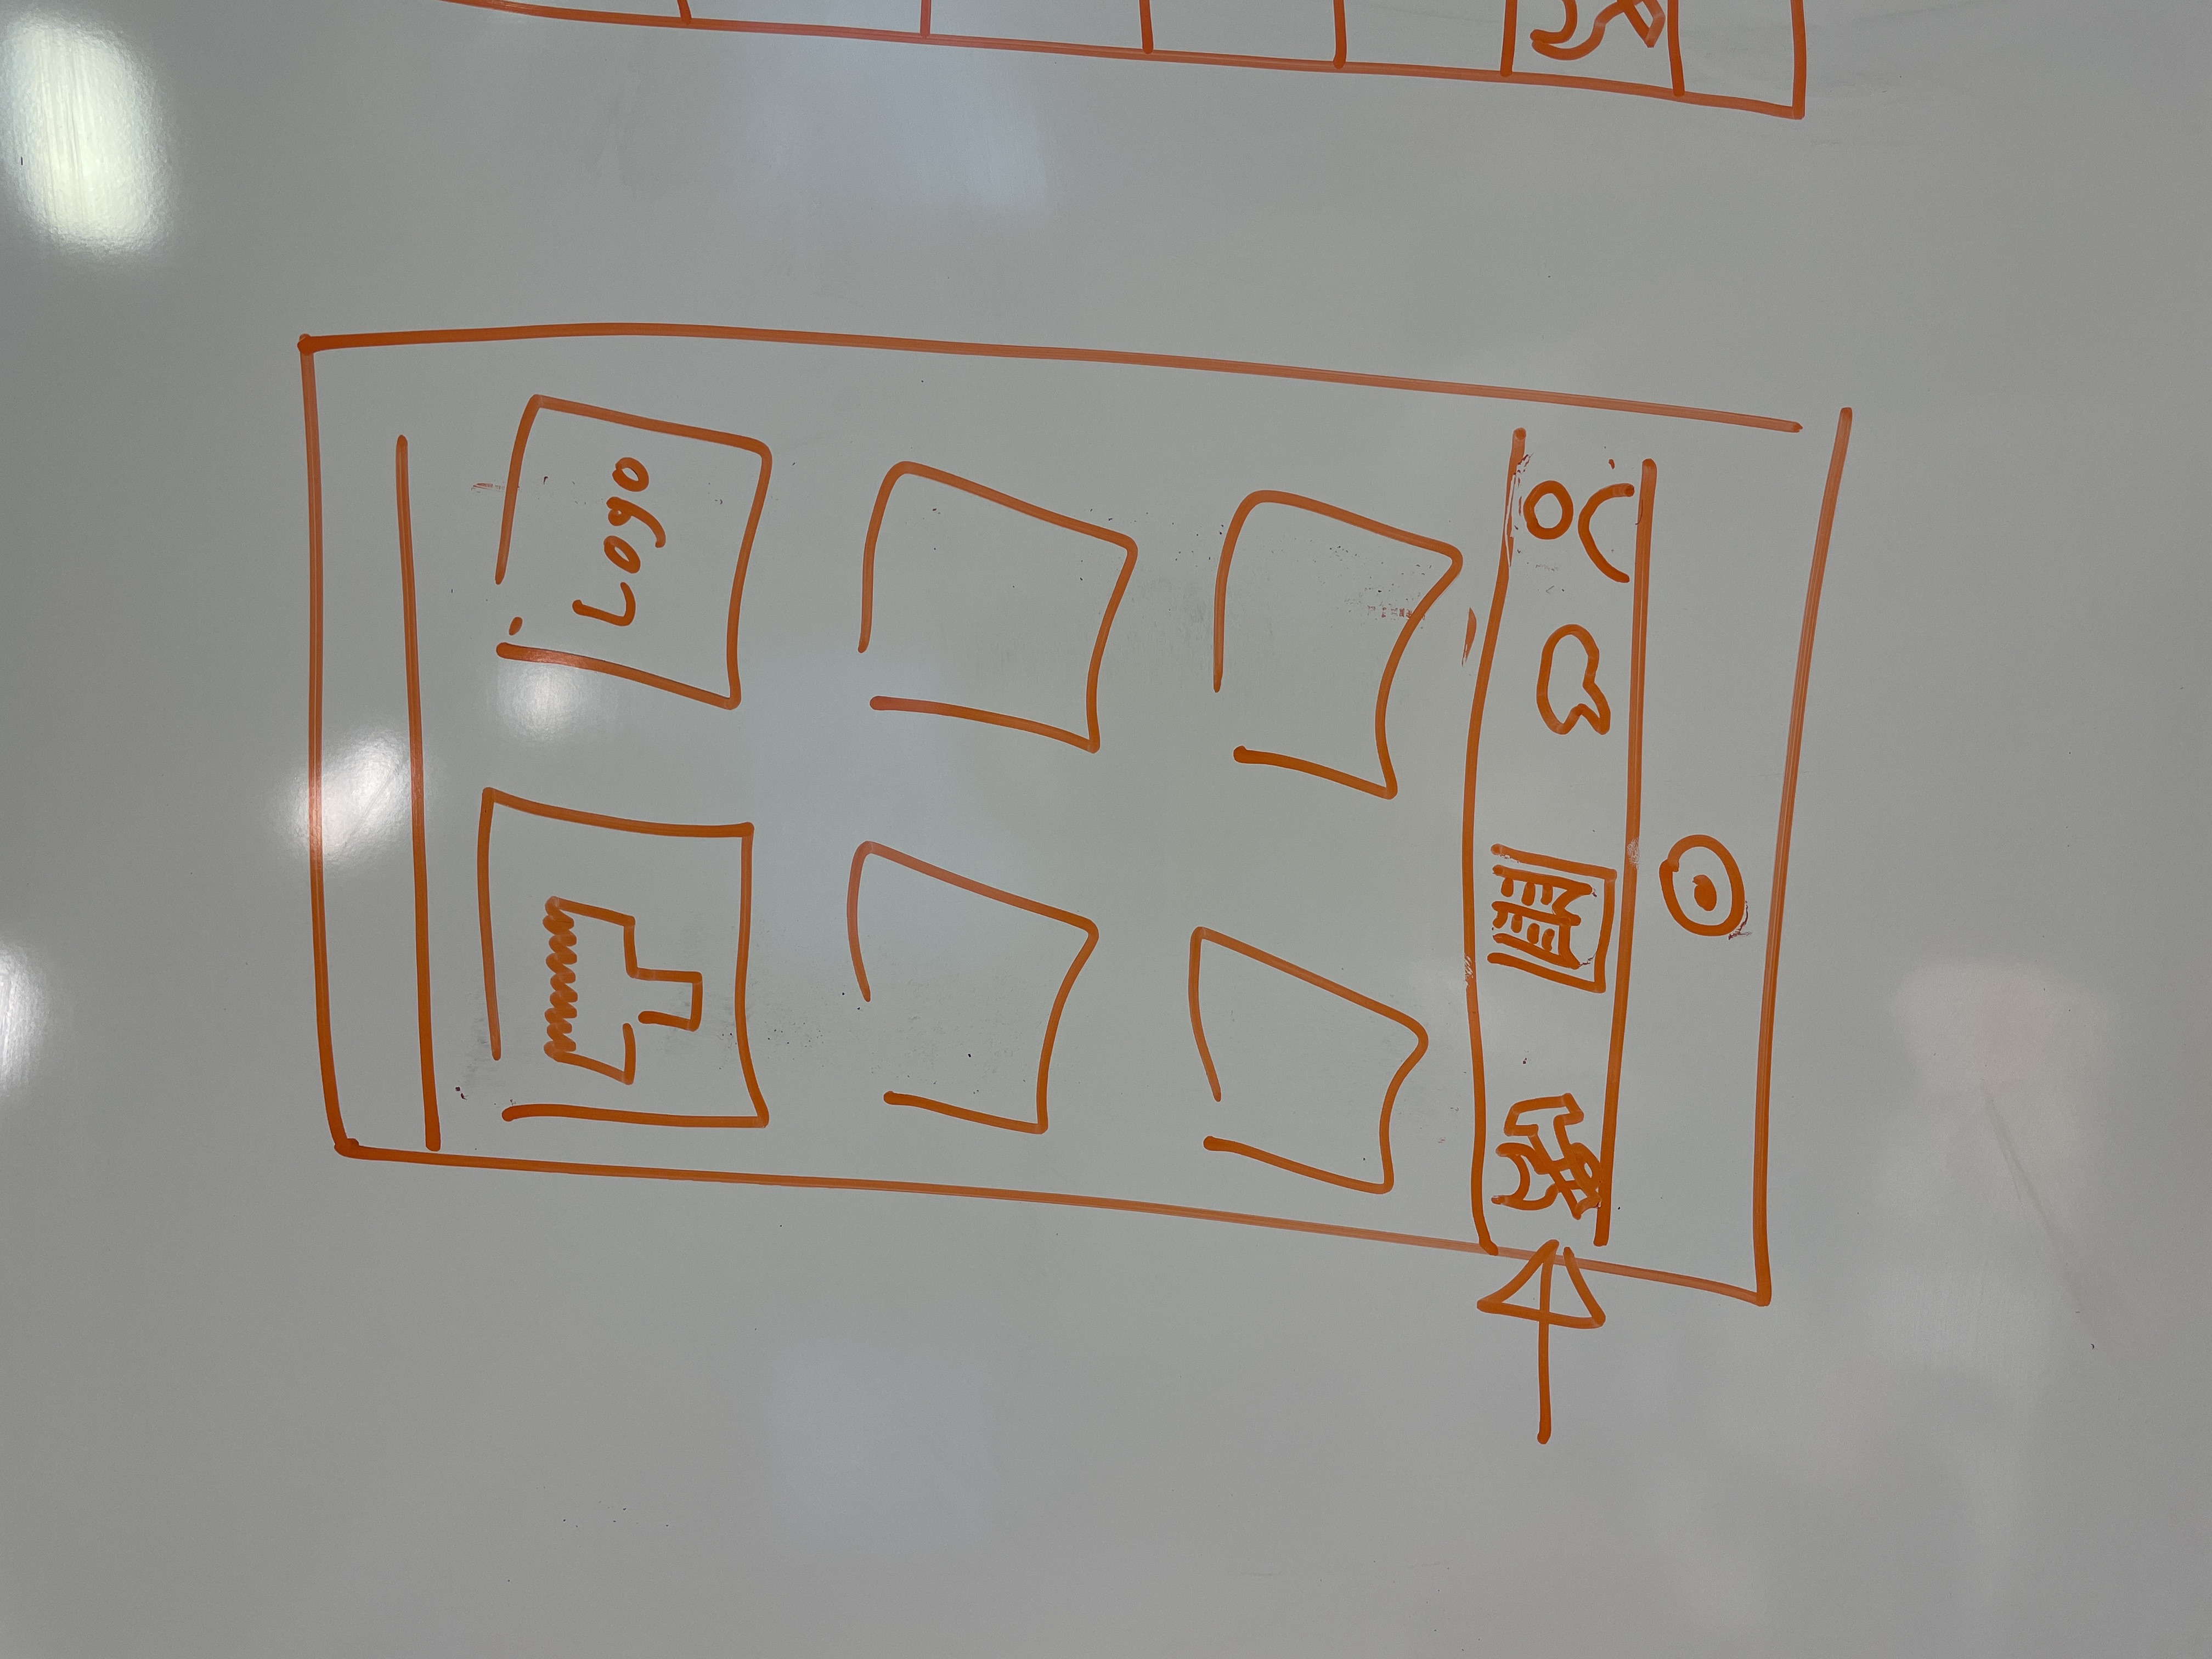
\includegraphics[angle=-90,width=6cm]{figures/home_pagina.jpg} }}%
    \qquad
    \subfloat[\centering job history]{{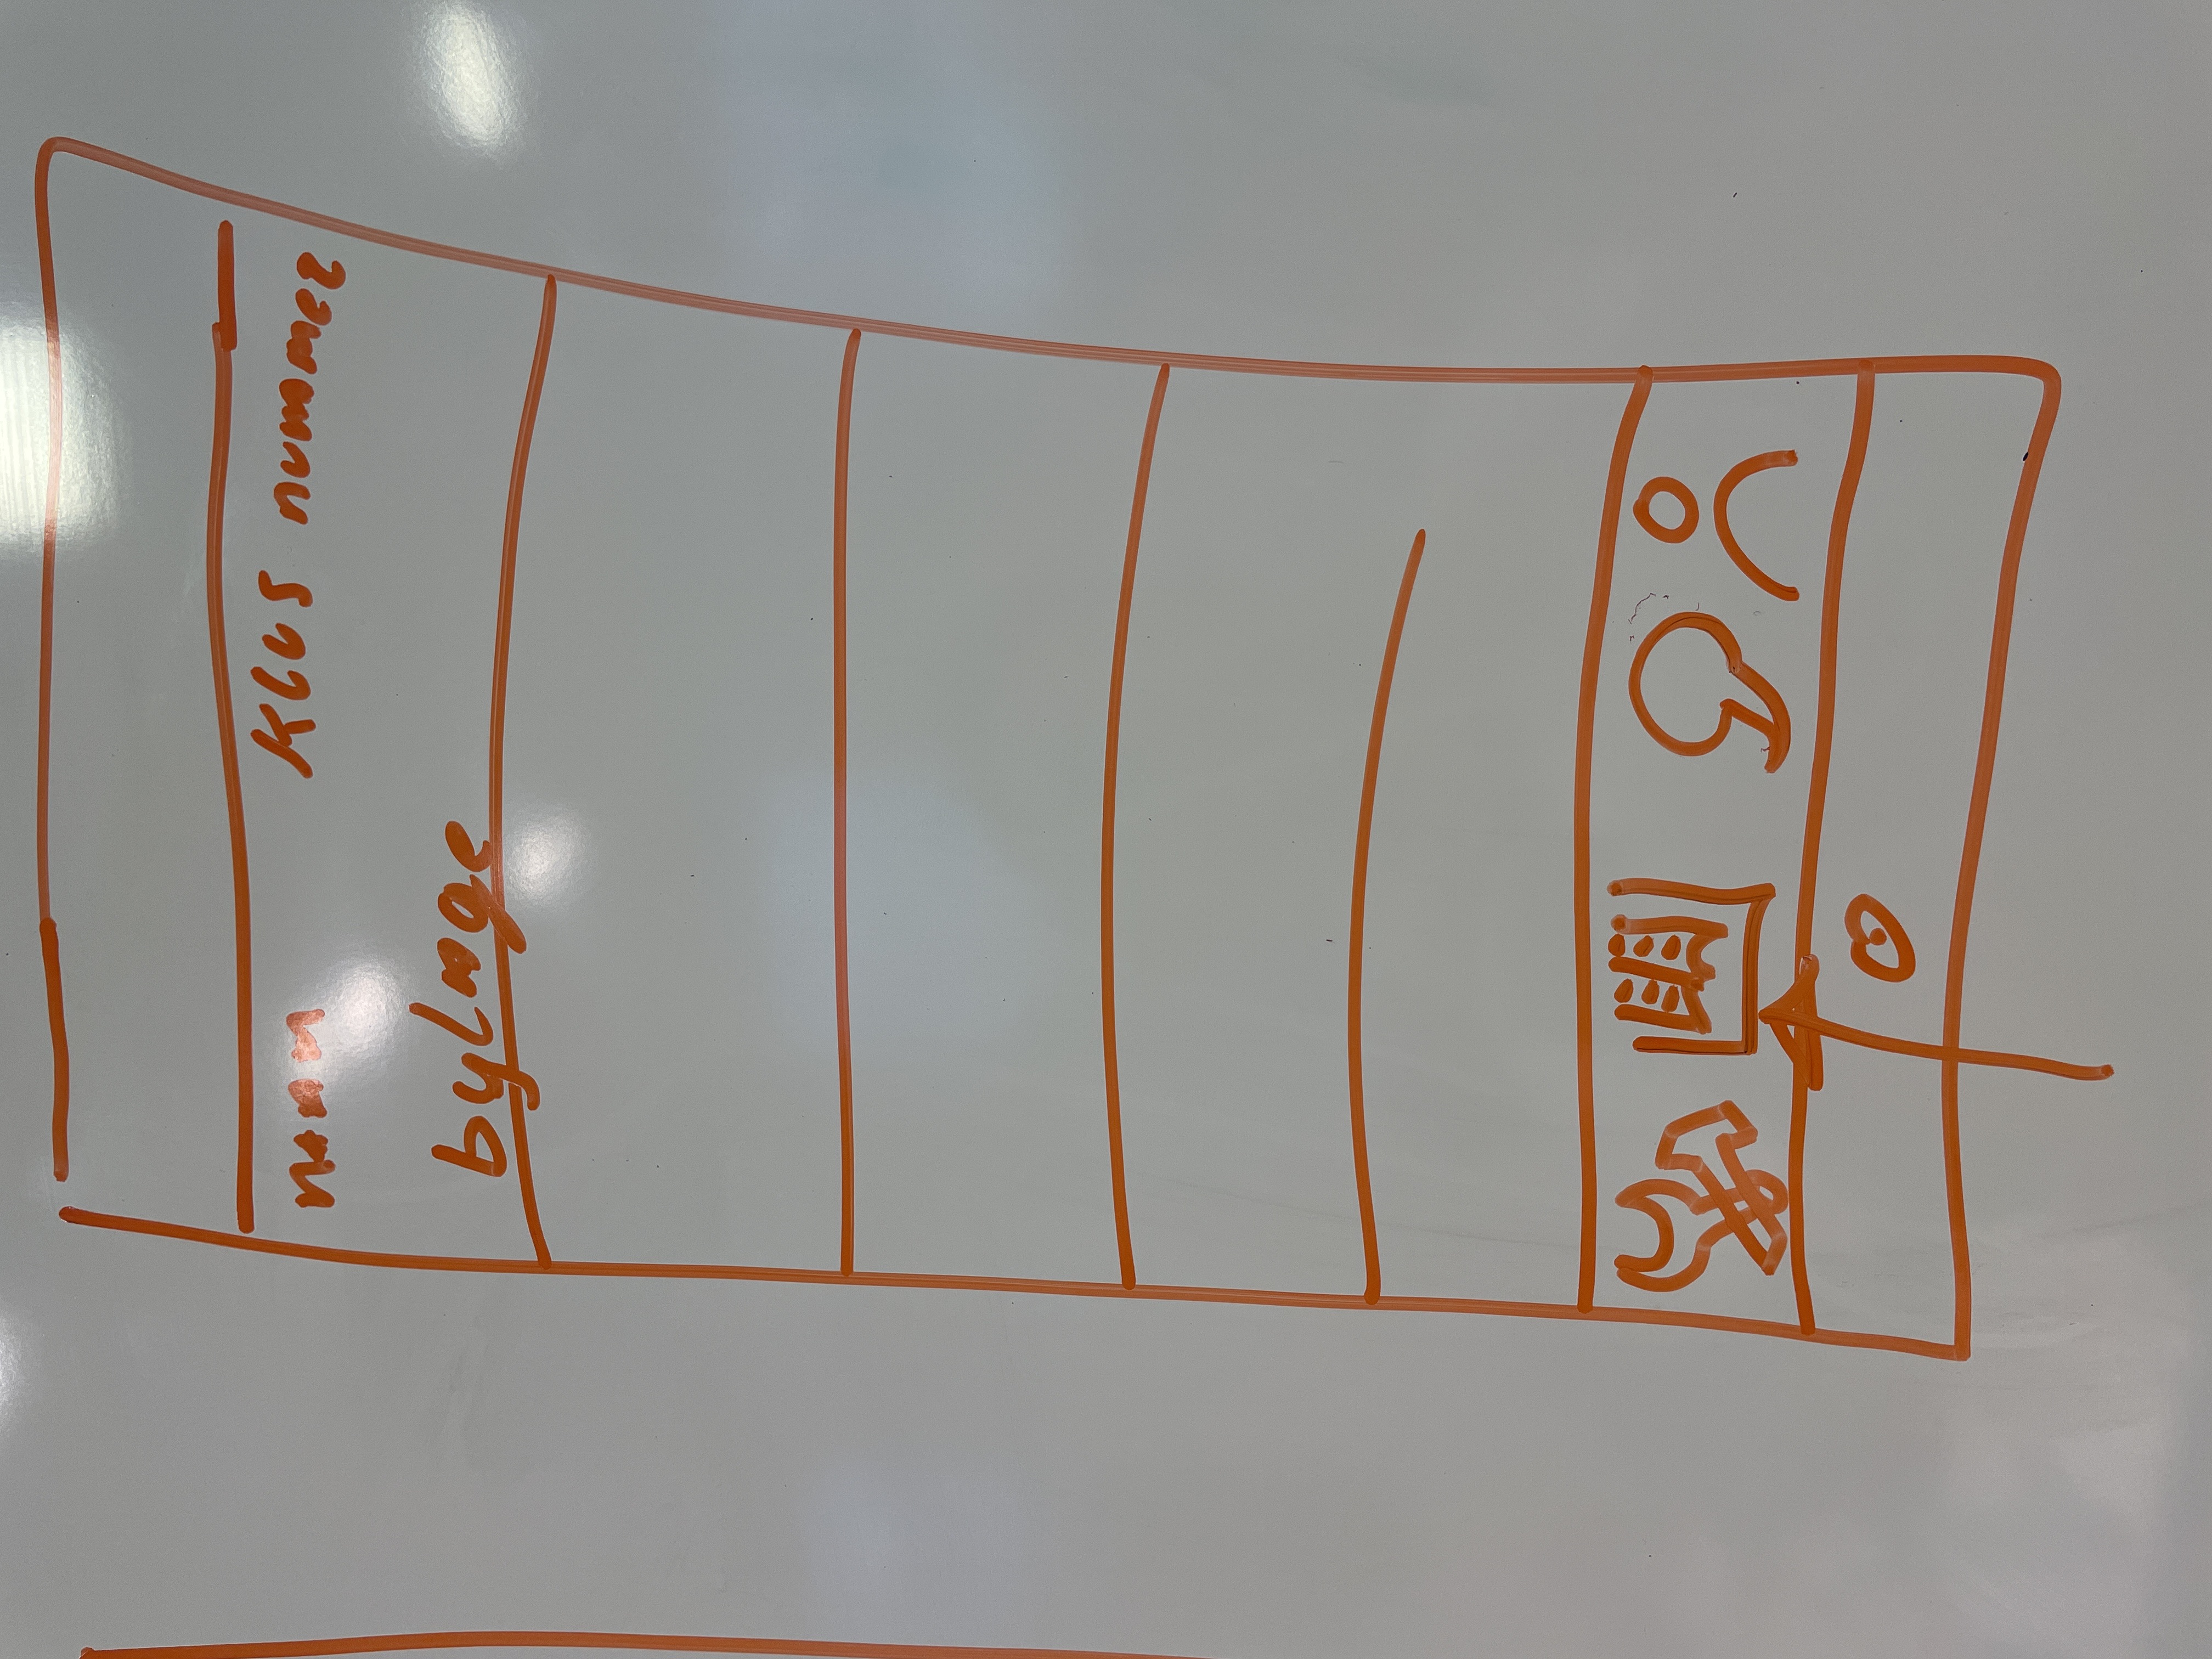
\includegraphics[angle=-90,width=6cm]{figures/booking.jpg} }}%

    \subfloat[\centering messaging]{{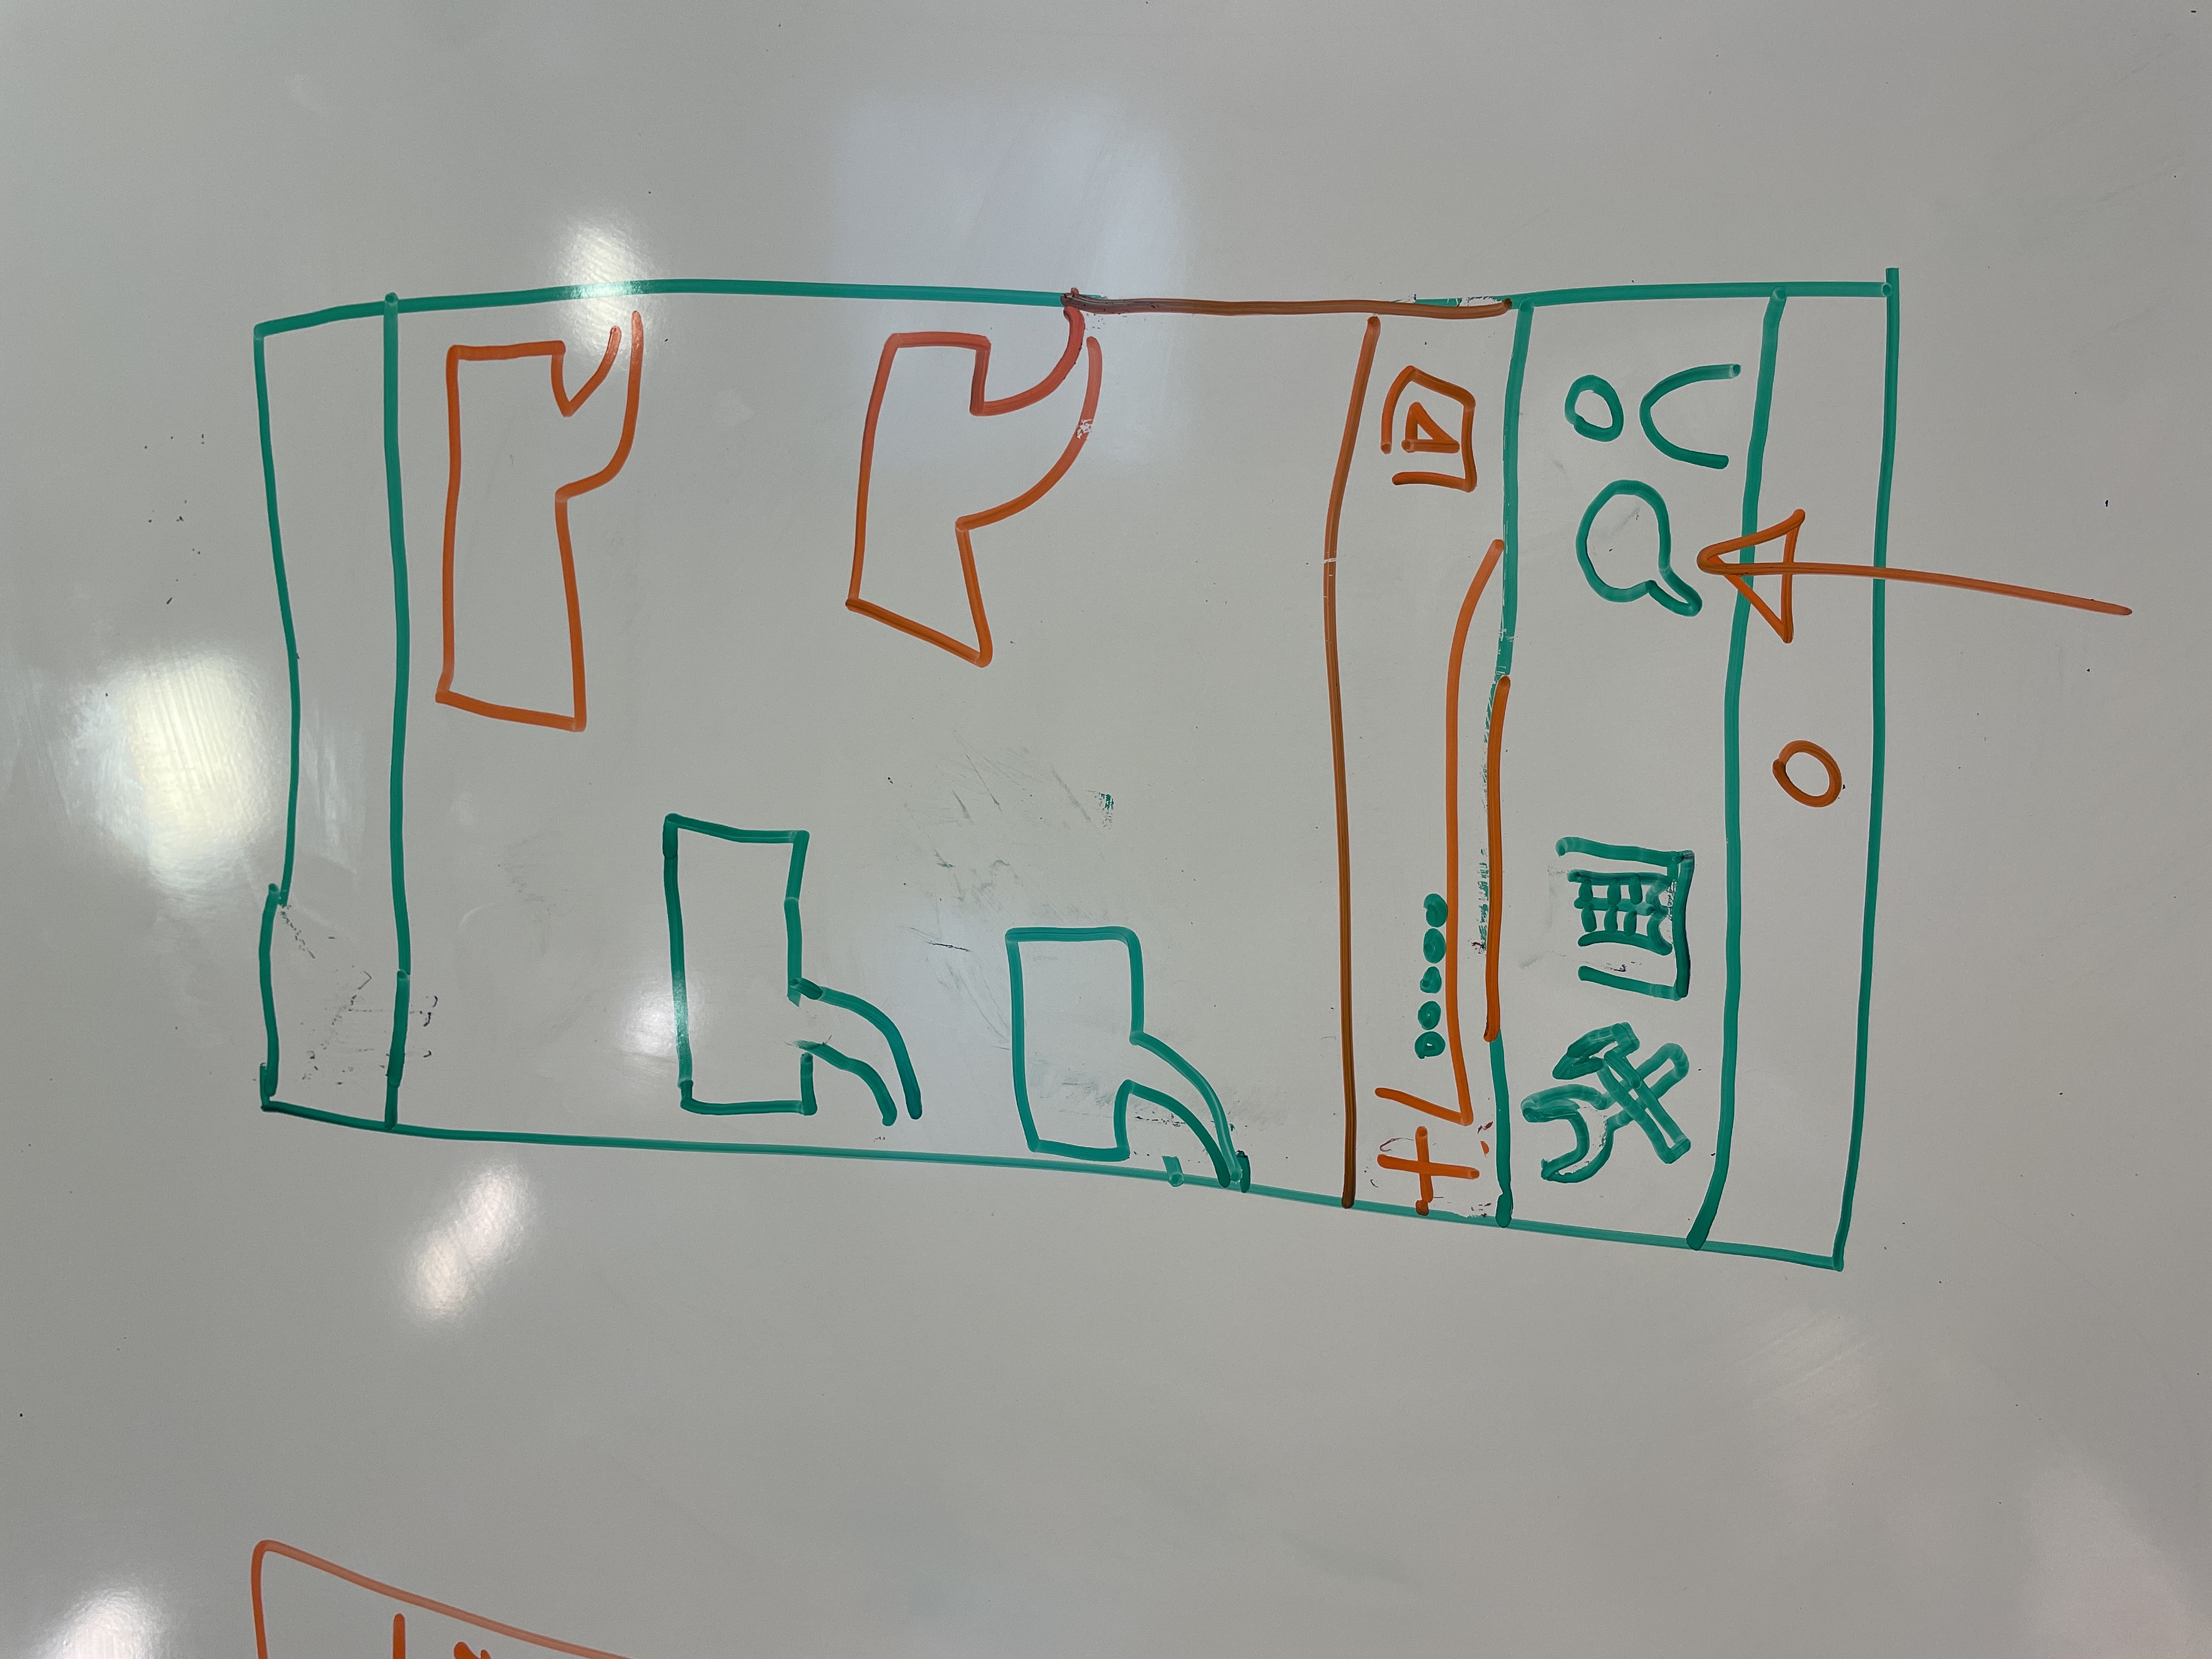
\includegraphics[angle=-90,width=6cm]{figures/messaging.jpg} }}%
    \qquad
    \subfloat[\centering profile]{{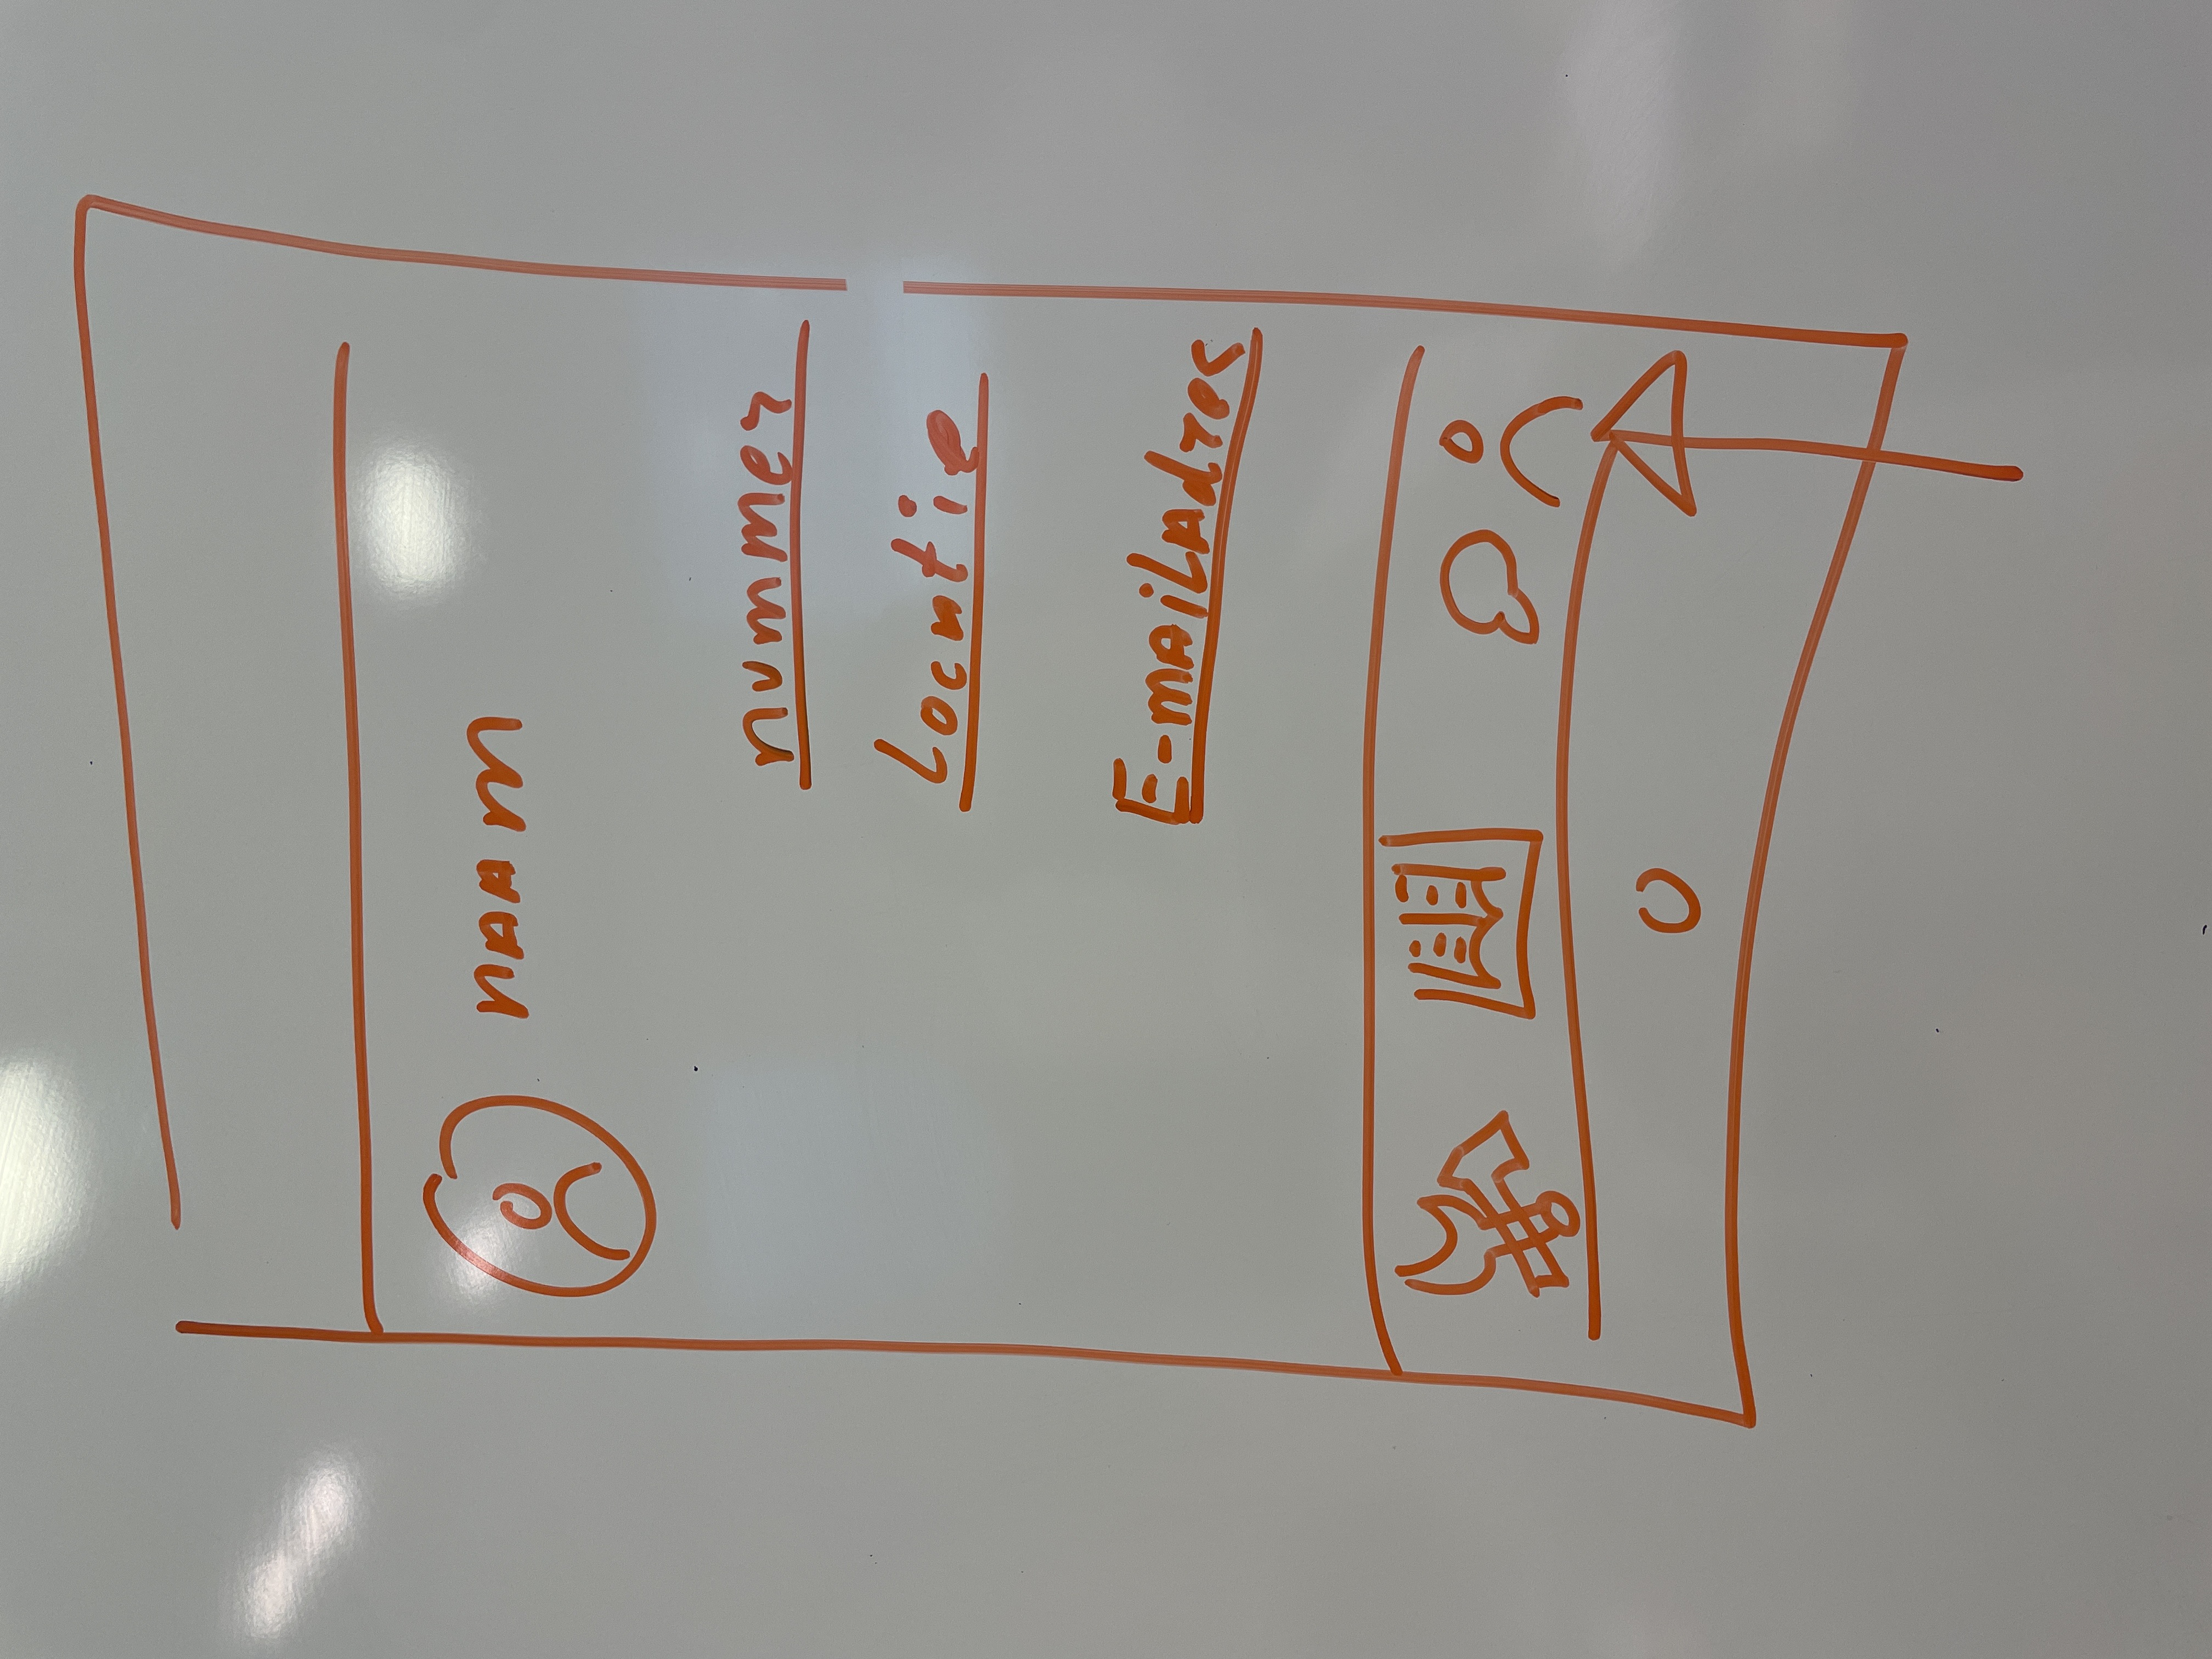
\includegraphics[angle=-90,width=6cm]{figures/profile.jpg} }}%
    \caption{Hand drawn wireframes of various sections of the app}%
    \label{fig:wireframes}%
\end{figure}

\section{Technical specifications}

Technologies that will likely be used to deliver the prototype are
PHP, HTML, JavaScript, CSS. For installing third-party libraries composer 
and/or NPM will be used. Third party tools for building effective graphical user
interfaces will likely include TailwindCSS and Bootstrap.

More details on each of these can be found here: 

\begin{table}[t]
	\centering
	\begin{tabular}{llll} 
		\toprule
		\textbf{Composer} & \url{https://getcomposer.org/} \\
		\textbf{NPM} & \url{https://www.npmjs.com/}\\
		\textbf{TailwindCSS} & \url{https://tailwindcss.com/} \\
		\textbf{Bootstrap} & \url{https://getbootstrap.com/} \\
	\end{tabular}
\end{table}


\end{document}
